%!TEX root = thesis.tex

\begin{figure}
\centering
                \scalebox{0.75}{
                    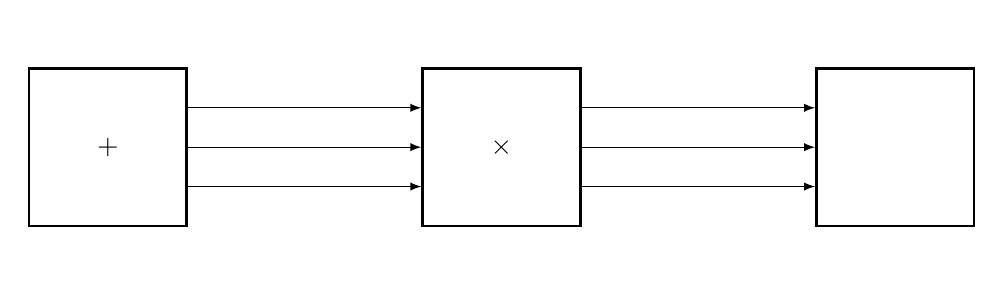
\begin{tikzpicture}
                        [
                            square/.style = {draw, shape=rectangle, minimum height=2cm, minimum width=2cm, node distance=2cm, line width=1pt},
                            empty/.style = {draw, shape=rectangle, minimum height=2cm, minimum width=2cm, node distance=2cm, line width=1pt, draw=white},
                        ]

                        \node[empty] (0a) at (0,0.5)     {};
                        \node[empty] (0b) at (0,-0.5)     {};
                        \node[square] (0c) at (0,0)     {$+$};

                        \node[empty] (1a) at (5cm,0.5)   {};
                        \node[empty] (1b) at (5cm,-0.5)   {};
                        \node[square] (1c) at (5cm,0)   {$\times$};

                        \node[empty] (2a) at (10cm,0.5)   {};
                        \node[empty] (2b) at (10cm,-0.5)   {};
                        \node[square] (2c) at (10cm,0)   {$\Enc$};

                        \draw [-latex] (0a.east) -- (1a.west);
                        \draw [-latex] (0b.east) -- (1b.west);
                        \draw [-latex] (0c.east) -- (1c.west);

                        \draw [-latex] (1a.east) -- (2a.west);
                        \draw [-latex] (1b.east) -- (2b.west);
                        \draw [-latex] (1c.east) -- (2c.west);

                    \end{tikzpicture}
                }
                \caption{A basic example of comopnent-based garbled circuits. In this figure, the 3 bit output of an addition component is linked into a multiplication component. The output of the multiplication component is then encrypted.}
                \label{fig:chaining-coarse}
            \end{figure}